%%%%%%%%%%%%%%%%%%%%%%%%%%%%%%%%%%%%%%%%%%%%%%%%%%%%%%%%%%%%%%%%%%%%%%%%
%                                                                      %
% LaTeX, FIIW thesis template                                          %
% 28/11/2014 v1.2                                                      %
%                                                                      %
%%%%%%%%%%%%%%%%%%%%%%%%%%%%%%%%%%%%%%%%%%%%%%%%%%%%%%%%%%%%%%%%%%%%%%%%
\documentclass[11pt,a4paper]{report}
% Indien je je thesis recto-verso wil afdrukken gebruik je onderstaande opties i.p.v. bovenstaande
%\documentclass[11pt,a4paper,twoside,openright]{report}

\usepackage[a4paper,left=3.5cm, right=2.5cm, top=3.5cm, bottom=3.5cm]{geometry}
\usepackage[english]{babel}
\usepackage{titlesec}

\usepackage{graphicx}
%\usepackage[latin1]{inputenc}           % om niet ascii karakters rechtstreeks te kunnen inputten
\usepackage[utf8]{inputenc}            % commentarieer deze regel uit als je utf8 encoded files gebruikt in plaats van latin1
\usepackage[numbers]{natbib}
\usepackage{listings}             		% voor het weergeven van broncode
\usepackage{verbatim}					% weergeven van code, commando's, ...
\usepackage[hidelinks]{hyperref}		% maak PDF van de thesis navigeerbaar without boxes
%\usepackage{hyperref}					% maak PDF van de thesis navigeerbaar
\usepackage{url}						% URL's invoegen in tekst met behulp van \url{http://}
\usepackage[small,bf,hang]{caption}     % om de captions wat te verbeteren
\usepackage[final]{pdfpages}            % gebruikt voor het invoegen van het artikel in pdf-formaat
\usepackage{pslatex}					% andere lettertype's dan de standaard types
\usepackage{lipsum}
\usepackage{sectsty}					% aanpassen van de fonts van sections en chapters
%\usepackage[nottoc,numbib]{tocbibind}	% Bibliography mee in de ToC
\usepackage{tikz}
\usepackage{xcolor}
\usepackage{standalone}
\usepackage{enumitem}
\usepackage{multirow}
\usepackage{chngpage}
% \usepackage{pdflscape}
\usepackage{rotating}
\setlist{nosep}
%\usetikzlibrary{external}

\allsectionsfont{\sffamily}
\chapterfont{\raggedleft\sffamily}

\usepackage{float}                      % De optie H voor de plaatsing van figuren op de plaats waar je ze invoegt. bvb. \begin{figure}[H]
%\usepackage{longtable}					% tabellen die over meerdere pagina's gespreid worden
%\usepackage[times]{quotchap}           % indien je fancy hoofdstuktitels wil
%\usepackage[none]{hyphenat}
%\usepackage{latexsym}
\usepackage{amsmath}
\usepackage{amssymb}

% MFA: zet zoekpad voor figure
\usepackage{subcaption}
\graphicspath{{fig/}}

\usepackage{fiiw_eng}

%door onderstaande regels in commentaar te zetten, of op false, kan je pagina's weglaten
%bijvoorbeeld het weglaten van een voorwoord, lijst met symbolen, ...
%%%%%%%%%%%%%%%%%%%%%%%%%%%%%%%%%%%%%%%%%%%%%%%%%%%%%%%%%%%%%%%%%%%%%%%%%%%%%%%%%%%%%%%%
%voorwoord toevoegen?
%\acknowledgementspagetrue
\acknowledgements{voorwoord}			%.tex file met daarin het voorwoord

%samenvatting toevoegen
%\summarypagetrue
\summary{samenvatting}					%.tex met daarin de samenvatting

%abstract toevoegen?
%\abstractpagetrue
\abstracts{abstract}					%.tex file met daarin het abstract
%lijst van figuren toevoegen?
%\listoffigurespagetrue
%lijst van tabellen toevoegen?
% \listoftablespagetrue
%lijst van symbolen toevoegen?
%\listofsymbolspagetrue
%\listofsymbols{symbolen}				%.tex file met daarin de lijst van symbolen



%informatie over het eindwerk, de promotor, ...
%%%%%%%%%%%%%%%%%%%%%%%%%%%%%%%%%%%%%%%%%%%%%%%
\opleiding{E-ICT}
\afdeling{Software Engineer - option ICT}

\campus{denayereng} %denayer,denayereng,geel,geeleng,gent,ghenteng,groept,groupteng,brugge,brugeseng

\title{Inverting knowledge graphs back to raw data}
\subtitle{How can we leverage the rules we use to construct knowledge graphs to do the inverse?}
% \author{naam student}
\forenameA{ }
\surnameA{ }


\forenameB{Tijs}
\surnameB{Van Kampen}

\academicyear{2023 - 2024}

\promotorA[Promotor]{Anastasia Dimou}
\promotorB[Co-Promotor]{}

\begin{document}
%\selectlanguage{dutch} %due to incompatible syntax with the English style library and the extended features of the dutch library, I'll be modifying the dutch library to be English
\selectlanguage{english} % For the English version
\preface

%%%%%%%%%%%%%%%%%%%%%%%%%%%%%%%%%%%%%%%%%%%%%%%%%%%%%%%%%%%%%%%%%%% 
%                                                                 %
%                            CHAPTER                              %
%                                                                 %
%%%%%%%%%%%%%%%%%%%%%%%%%%%%%%%%%%%%%%%%%%%%%%%%%%%%%%%%%%%%%%%%%%% 

\chapter{Thesis details}

\textbf{Title: } Inversion: from knowledge graphs to raw data

\textbf{Subject: } 
\begin{itemize}
	\item \textbf{RQ1: } How can we leverage RML to construct raw data from heterogeneous data.
	\item \textbf{RQ2: } How can we extend an existing system like RML or create a new system to construct raw data from knowledge graphs.
\end{itemize}

\begin{description}
	\item[Description:] Knowledge graphs are gaining traction nowadays and more and more companies use them, such as Amazon, Bosch, IKEA, Facebook, Google, LinkedIn, SIEMENS, Zalando, etc. Most knowledge graphs are nowadays constructed from other heterogeneous data sources, such as tables in relational databases, data in XML files or in JSON format derived from a Web API. While the construction of knowledge graphs from heterogeneous data was theoroughly investigated so far, the inverse, namely constructing raw data from knowledge graphs is not explored so far. \newline Initially we will investigate reconstructing tables back to their initial form from an RDF graph, later extending this to other formats like JSON, XML,...
\end{description}

\textbf{Company: } internal research group EAVISE, CAMPUS DE NAYER

\textbf{University promotor: } Anastasia Dimou

\textbf{Planning: } See gantt chart in figure \ref{fig:gantt_chart} for a visual overview.

Goals/Deadlines:
\begin{itemize}
	\item \textbf{22nd October: } Gathering information 
	\begin{itemize}
		\item Defining the problem
		\item Refine research questions
	\end{itemize}
	\item \textbf{12th November: } Write related work
	\item \textbf{3th December: } Prototype
	\item \textbf{22nd December(deadline intermediate report): } Expand and improve related work
	\item \textbf{3th March: } Implementation
	\item \textbf{5th May: } Evaluation and refining implementation
	\item \textbf{4th June(deadline final report): } Finalize report
\end{itemize}


\begin{sidewaysfigure}[htbp]
	\centering
	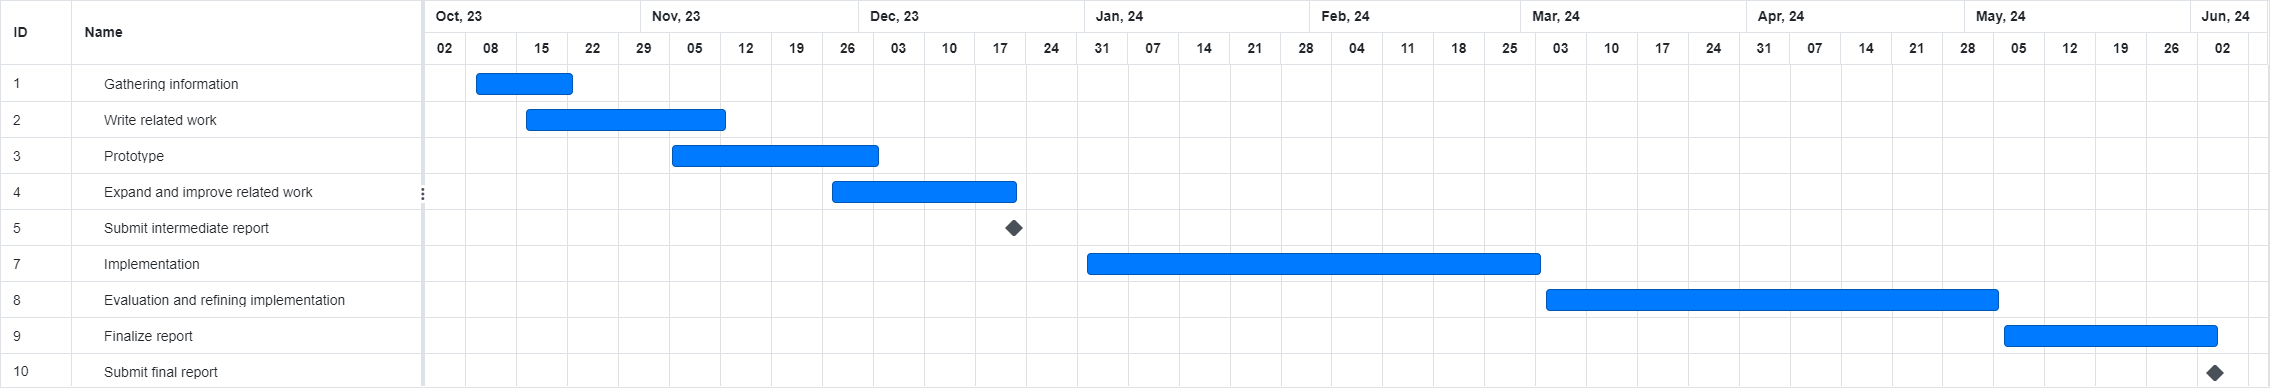
\includegraphics[width=\pdfpagewidth]{fig/startup_report/gantt_final.png}
	\caption{Gantt chart}
	\label{fig:gantt_chart}
\end{sidewaysfigure}
% Bibliografie: referenties. De items zitten in bibliografie.bib
%%%%%%%%%%%%%%%%%%%%%%%%%%%%%%%%%%%%%%%%%%%%%%%%%%%%%%%%%%%%%%%%%
% Indien je ook de niet geciteerde werken in je bibliografie wil opnemen, commentarieer dan onderstaande regel uit!
%\nocite{*}
\bibliographystyle{plainnat}
%\bibliography{bibliografie}

% Eventueel enkele appendices
%%%%%%%%%%%%%%%%%%%%%%%%%%%%%%
%\appendix
%%%%%%%%%%%%%%%%%%%%%%%%%%%%%%%%%%%%%%%%%%%%%%%%%%%%%%%%%%%%%%%%%%% 
%                                                                 %
%                            CHAPTER                              %
%                                                                 %
%%%%%%%%%%%%%%%%%%%%%%%%%%%%%%%%%%%%%%%%%%%%%%%%%%%%%%%%%%%%%%%%%%% 



\end{document}

% Back cover: change according to the correct campus
%
\includepdf{private/back_fiiw_denayer.pdf}

\includepdf{private/back_fiiw_denayer_eng.pdf} % For the English version
%
\includepdf{private/back_fiiw_geel.pdf}
% \includepdf{private/back_fiiw_geel_eng.pdf} % For the English version
%
\includepdf{private/back_fiiw_gent.pdf}
% \includepdf{private/back_fiiw_ghent_eng.pdf} % For the English version
%
\includepdf{private/back_fiiw_brugge.pdf}
% \includepdf{private/back_fiiw_bruges_eng.pdf} % For the English version
%
\includepdf{private/back_fiiw_groept.pdf}
% \includepdf{private/back_fiiw_groupt_eng.pdf} % For the English version

% \end{document}